\documentclass[a4paper,10pt]{book}
\usepackage[utf8x]{inputenc}
\usepackage[english,russian]{babel}
\usepackage{graphicx} 

\usepackage{geometry} % Меняем поля страницы
\geometry{left=2cm}% левое поле
\geometry{right=1.5cm}% правое поле
\geometry{top=1cm}% верхнее поле
\geometry{bottom=2cm}% нижнее поле

\renewcommand{\theenumi}{\arabic{enumi}}% Меняем везде перечисления на цифра.цифра
\renewcommand{\labelenumi}{\arabic{enumi}}% Меняем везде перечисления на цифра.цифра
\renewcommand{\theenumii}{.\arabic{enumii}}% Меняем везде перечисления на цифра.цифра
\renewcommand{\labelenumii}{\arabic{enumi}.\arabic{enumii}.}% Меняем везде перечисления на цифра.цифра
\renewcommand{\theenumiii}{.\arabic{enumiii}}% Меняем везде перечисления на цифра.цифра
\renewcommand{\labelenumiii}{\arabic{enumi}.\arabic{enumii}.\arabic{enumiii}.}% Меняем везде перечисления на цифра.цифра

\usepackage{hyperref}

\begin{document}


\begin{titlepage} % Титульный лист
\newpage\vspace*{\fill}




\begin{center}

\textsc{\textbf{\Large GdbOF: Инструмент отладки для $OpenFOAM^{\tiny\textcircled{R}}$}} \\
\vspace{2.5em}
Juan M. Gim\'enez\hspace{6em} Santiago M\'arquez Dami\'an \\
Norberto M. Nigro \\
\small Международный Центр Вычислительных Методов в Инженерии (CIMEC), \\
INTEC-UNL/CONICET, \\
G\"uemes 3450, Santa Fe, Argentina, http://www.cimec.org.ar\\
Ноябрь 10, 2011\\


\end{center}

\vspace*{\fill}\newpage


\end{titlepage}


\tableofcontents % это оглавление, которое генерируется автоматически


\chapter*{Введение}
\addcontentsline{toc}{chapter}{Введение}


Библиотеки $OpenFOAM^{\tiny\textcircled{R}}$ великий вклад в CFD сообщество и мощное средсво для создания
решателей и других инструментов. Тем не менее в этом творческом процессе требуются глубокие знания о структуре классов,
как для хранения данных о геометрии так и для матриц, получающихся из систем уравнений, что становится предпосылкой для
отладки программы - дебаггинга. \\
gdbOF это новый инструмент, на основе gdb (GNU Debugger) который позволяет анализировать структуры классов во время
отладки. Это приложение состоит из gdb макросов, эти макросы обращаются к коду классов и непосредственно к данным, таким образом,
запрашивая информацию. Данное руководство описывает ключевые моменты данного инструмента, включая различные примеры такие как
сборка и хранение матриц в скалярной адвективной-диффузионной задаче, неортогональные методы корекции в чисто диффузионных тестах и
мультифазовые решатели основанные на методе объёма жидкости (Volume of Fluid). В этих тестах рассматриваются несколько типов
данных, такие как внутренний и граничный вектор и скалярные значения полей решения, потоки на поверхностях ячеек, граничные патчи
и граничные условия. Как дополнительные возможности описаны сброс данных в файл и графический просмотр. \linebreak
Все эти возможности делают gdbOF применимым не только в академических тестах, но также в реальных задачах.

                                                                                                            

\chapter{Требования и установка}

...

\chapter{Основы отладки}
Наиболее распространённая операция в процессе отладки - посмотреть значения, хранящиеся в массиве, это делается в gdb командой как
показано в Примере 1, где \texttt{v} это анализируемый массив.
\vspace{2 mm}

\hrule\smallskip
\textbf{Пример 1} Содержимое массива.
\smallskip\hrule
\vspace{2 mm}
\texttt{\$(gdb) p *v@v\_size}
\vspace{2 mm}
\smallskip\hrule
\vspace{2 mm}

Когда требуется проанализировать атрибуты класса, необходимо знать дерево наследования классов. Это позволит обращаться
к классам, которые содержат другие классы, как к атрибутам. Для получения данной информации необходимо пройтись по указателям
чтобы найти интересующий атрибут. Типичный пример, когда требуется проверить во время отладки, что некое граничное условие
удовлетворяет условию (обычно когда граничное условие задано непосредственно в решателе и информация о поле получается после решения
первого временного шага). Граничные условия в $OpenFOAM^{\tiny\textcircled{R}}$ задаются для каждого патча в \texttt{GeometricField},
 затем, полагая, что патч имеет индек 0 (атрибут \texttt{BoundaryField} содержит информацию обо всех патчах), рассмотрим значения
получаемые из выражения патча, как показано в Примере 2, где \texttt{vSF} это \texttt{volScalarField}.

\vspace{2 mm}
\hrule\smallskip
\textbf{Пример 2} Просмотр значений Boundary Field.
\smallskip\hrule
\vspace{2 mm}
\texttt{\$(gdb) p *(vSF.boundaryField\_.ptrs\_.v\_[0].v\_) \\
\hspace*{15 mm}@(vSF.boundaryField\_.ptrs\_.v\_[0].size\_)}
\vspace{2 mm}
\smallskip\hrule
\vspace{2 mm}

Обратите внимание что выражение в Примере 2 не включает какие либо обращения к встраиваемым inline функциям, которые могли бы
привести к некоторым проблемам в gdb\footnote{Встраиваемые inline функции это оптимизация, при которой при каждом вызове
функции вставляется тело её копии вместо ссылки на одну и ту же функцию. gdb отображает inline функции как не-inline функции.
Чтобы inline функция заработала в gdb, компилятор обязан записать информацию о вставке в отладочную информацию. gcc использует
формат dwarf 2, чтобы делать это как некоторые другие компиляторы. С другой стороны gdb только поддерживает inline функции согласно
dwarf 2. В версиях gcc до 4.1 не было двух требуемых атрибутов (DW\_AT\_call\_file и DW\_AT\_call\_line), поэтому gdb не отображает
inline функции в ранних версиях gcc.}, предоставляя более сложный доступ к информации.

\vspace{2 mm}

\textit{gdbOF} разрешает неудобства, связанные с знанием расположения атрибута и использованием длинных выражений. Используя \textit{gdbOF}
команды, как это показано в Примере 3, можно достичь тех же результатов. Обратите внимание на упрощение выражения, благодаря \textit{gdbOF},
объём работ сократился и для выполнение тех же заданий стало проще и понятнее.
Дополнительные свойства позволяют определять пределы вывода. Выбирая начальный и конечный индексы можно задать диапазон вывода желаемых
значений. В \textit{gdbOF} команда называется \texttt{ppatchvalueslimits} (схожая команда называется \texttt{pinternalvalueslimits}).

\vspace{2 mm}
\hrule\smallskip
\textbf{Пример 3} Просмотр значений Boundary Field с помощью \textit{gdbOF}.
\smallskip\hrule
\vspace{2 mm}
\texttt{\$(gdb) ppatchvalues vSF 0}
\vspace{2 mm}
\smallskip\hrule
\vspace{5 mm}

В Псевдокоде 1 представлена схема работы команды.

\vspace{5 mm}
\hrule\smallskip
\textbf{Псевдокод 1} Структура команд \texttt{ppatchvalueslimits} и \texttt{pinternalvalueslimits} в \textit{gdbOF}.
\smallskip\hrule
\vspace{2 mm}
\small {\begin{enumerate}
         \item Получение параметров: название поля, пределы и patchindex (только для patchvalueslimits)
	 \item Подтверждение пределов для вывода
	\item Определение типа поля (объём-поверхность или скаляр-вектор-тензор)
	\item вывод значений поля в соответствующем формате

        \end{enumerate}
}
\vspace{2 mm}
\smallskip\hrule
\vspace{2 mm}

Есть много примеров в $OpenFOAM^{\tiny\textcircled{R}}$ в которых как и в предыдущем необходимость в инструменте, который
упрощает доступ к сложной диаграмме классов должна быть обудмана. Заметьте что в предыдущем примере не описывалось как определяется
индекс желаемого патча. Обычно пользователь знает только строку, которая определяет патч, но не индекс по которому он расположен
в списке патчей. Здесь \textit{gdbOF} снова приходит на помощь, предоставляя команду, которая отображает список патчей с  
соответствующим индесом. Используется команда представленная в Примере 4.

\vspace{2 mm}
\hrule\smallskip
\textbf{Пример 4} Просмотр списка патчей с помощью \textit{gdbOF}.
\smallskip\hrule
\vspace{2 mm}
\texttt{\$(gdb) ppatchlist}
\vspace{2 mm}
\smallskip\hrule
\vspace{5 mm}

Другой важный момент - учесть во время отладки и монитор истинности переменных или экземпляров классов. Чтобы просмотреть значения
поля или системы уравнений необходимо поставить gdb оператор \textit{break} в строке относящейся к отображению анализируемой
переменной. Для этого требуется проанализировать код - до отладки, или хотябы распознать объекты, чьи переменные будут проверяться.
Здесь $OpenFOAM^{\tiny\textcircled{R}}$ создаёт дополнительную сложность из-за применения в коде \textit{макро C++ функций},
в которые gdb не может вставить \textit{break}. Поэтому чтобы просмотреть переменные, определённые в мониторе, требуется
перепрыгивать по коду используя команды \textit{step}, \textit{next} и \textit{finish}.

\vspace{2 mm}

Выше было лишь описание задач и тоо как инструмент упрощает отладочную работу. Для более глубокого изучения \textit{gdbOF} макросов,
\textit{gdbOF} документация содержит ценные ссылки.

\chapter{Расширенная отладка}

\section{Матрица системы}
\label{sec:3.1}
С увеличением сложности отладки появляются кейсы, в которых не просто находится атрибут и пересылается в решение задачи. Обычный кейс
представляет собой систему, \textit{Ax=b}, получаемую дискретизацией системы дифференциальных уравнений которая решается и сохраняется
с помощью технологии \textit{LDUAddressing} (смотри Приложение \nameref{sec:PrilA}). Эта технология имеет преимущество для матриц
в разряженном формате и просто хранит коэффициенты. Этот формат хранения и необходимость доступа и пересылки значений требует
выводить значения по одному на каждом шагу, для перевода матрицы в желаемый формат. Для такой задачи есть две команды, одна для невырожденных
и другая для вырожденных матриц.

Чтобы выполнить необходимые циклы по элементам матрицы, gdb использует C-образный синтаксис для выполнения итерационных (while, do-while) и
структур с условием (if, else). Эти команды имеют очень низкую производительность, поэтому итерации по большим блокам данных должны быть
выполненны отдельно. \textit{gdbOF} становится независимым от gdb при работе с матрицами с помощью другой платформы: \texttt{lduAddressing}
векторы экспортируются во внешние файлы с которыми далее работают через вызовы к оболочке вычислений выполняемых на другом языке.
В \textit{gdbOF}, python выбран из-за его возможности запускать скрипты из консоли и простого управления файлами, как для загрузки так 
и для сохранения данных.

Должнобыть неудобно, что макросы \textit{gdbOF} для массивов имеют более сложные опции включая не только просмотр полной матрицы (M x N), но
подматрицы определённые парой начала [\textit{row,col}] и парой конца [\textit{row,col}]. Согласно коду, не требуется больше заботиться
в определении границ цикла, который переупорядочивает матрицу. Следующая диаграмма поясняет как работает команда \texttt{pfvmatrixfull}
(с ограничениями или без) как показано в Псевдокоде 2 и диаграмма для команды \texttt{pfvmatrixsparse} (с ограничениями или без) как показано
в Псевдокоде 3.

\section{Работа с сеткой}
\label{sec:3.2}

Другая группа макросов занимается операциями с сеткой. Вышеупомянутый проблема gdb при выполнении циклов над большими блоками данных,
 в том числе 
в случае сеток, заставляет искать для этой задачи внешние инструменты. Учитывая достоинство библиотеки $OpenFOAM^{\tiny\textcircled{R}}$ как
содержащей набор методов для выполнения этих задач, \textit{gdbOF} использует создание автономных приложений к которым обращается во 
время отладки для выполнения задачи. Даже не смотря на то, что этот способ подразумевает создание новых экземпляров сетки в памяти,
 стоимость времени и разработки ниже, чем потребовалось бы для управления работой с сеткой в gdb, используя циклы gdb с C-образным 
синтаксисом или на другом языке, например python. Эти $OpenFOAM^{\tiny\textcircled{R}}$ приложения включены в пакет \textit{gdbOF} и 
скомпилированы, вместе с запуском установщика \textit{gdbOF}.

\vspace{2 mm}
\hrule\smallskip
\textbf{Псевдокод 2} Структура комманды \textit{gdbOF} \texttt{pfvmatrixfull}.
\smallskip\hrule
\vspace{2 mm}
\small {\begin{enumerate}
        \item Получение параметров
	\item Получение верхнего и нижнего массивов с помощью gdb
	\item Перенаправление данных во внешний файл
	\item Перевод формата внешних файлов из gdb формата в python формат
	\item Вызов python скрипта для обработки матрицы
	\begin{enumerate}
		\item[(a)] Прочитать внешние файлы
		\item[(b)] Установить пределы
		\item[(c)] Произвести lduAddressing (смотри \nameref{sec:PrilA})
		\item[(d)] Заполнить нолями
	\end{enumerate}
	\item Перевод формата внешних файлов из python формата в gdb формата
	\item Показать в выводе и сохранить файл в восьмеричном формате
        \end{enumerate}
} 
\vspace{2 mm}
\smallskip\hrule
\vspace{5 mm}


\vspace{2 mm}
\hrule\smallskip
\textbf{Псевдокод 3} Структура комманды \textit{gdbOF} \texttt{pfvmatrixsparse}.
\smallskip\hrule
\vspace{2 mm}
\small {\begin{enumerate}
        \item Получение параметров
	\item Получение верхнего и нижнего массивов с помощью gdb
	\item Перенаправление данных во внешний файл
	\item Перевод формата внешних файлов из gdb формата в python формат
	\item Вызов python скрипта для обработки матрицы
	\begin{enumerate}
		\item[(a)] Прочитать внешние файлы
		\item[(b)] Произвести lduAddressing для разреженной матрицы
		\item[(d)] Сгенерировать заголовок разреженного файла
	\end{enumerate}
	\item Перевод формата внешних файлов из python формата в gdb формата
	\item Показать в выводе и/или сохранить файл в восьмеричном формате с добавлением заголовка к телу файла
        \end{enumerate}
} 
\vspace{2 mm}
\smallskip\hrule
\vspace{5 mm}

Случаи поиска по сетке обычно покрываемые \textit{gdbOF} те, которые начинаются с точки определяемой [\textit{x,y,z}],
возвращают индекс или значение ячейки некоторого поля, и то и другое в центре ячейки (volFields) или в каждом его поверхности (surfaceFields).

Что касается получения значения поля в некоторой точке это не более неудобно чем нахождение индекса ячейки или индекса ячейки, содержащей
точку, чей центроид ближайший к ней. Чтобы это сделать \textit{gdbOF} использует обращение к одному из приложений которые компилируются
во время установки, но пользователю нужен только вызвать простую команду показанную в Примере 5 (раздел \ref{Prim5}), где \texttt{x,y} и \textit{z} параметры
задаваемые пользователем в командном вызове представляющие (\textit{x,y,z}) координаты точки. Команда возвращает два индекса: индекс ячейки,
содержащей точки и индекс ячейки, центроид которой ближайший. Затем пользователь заполняет один из этих индексов в команде
 \texttt{pinternalvalueslimits} для извлечения значения поля в центроид ячейки или чтобы проверить уравнение заданное для данной ячейки
командой \texttt{pfvmatrix}.

Псевдокод этого инстумента представлен в Псевдокоде 4, обратите внимание он нет коммуникации между gdb и другими платформами кроме
вызова оболочки.

\vspace{2 mm}
\hrule\smallskip
\textbf{Пример 5}\label{Prim5} Просмотр индекса ячейки.
\smallskip\hrule
\vspace{2 mm}

\texttt{\$(gdb) pfindCell x y z}

\vspace{2 mm}
\smallskip\hrule
\vspace{5 mm}

Возврат результатов через временные файлы, которые должны быть сгенерированы в соответствующем формате, чтобы быть читаемыми для \textit{gdbOF}.
Эта техника используется потомучто не возможно получить доступ к значениям в памяти из одного процесса другому процессу.

\vspace{2 mm}
\hrule\smallskip
\textbf{Псевдокод 4}\label{Prim5} Структура комманды \textit{gdbOF} \texttt{pfindcell}.
\smallskip\hrule
\vspace{2 mm}

{\begin{enumerate}
        \item Получение параметров
	\item Вызов приложения FOAM для создания поиска
	\begin{enumerate}
		\item[(a)] Запуск нового кейса
		\item[(b)] Произвести поиск (как описано в \nameref{sec:PrilC})
		\item[(d)] Сохранить результаты во временный файл
	\end{enumerate}
	\item Прочитать временный файл с помощью скрипта оболочки
	\item Показать индексы в стандартном выводе
        \end{enumerate}
} 

\vspace{2 mm}
\smallskip\hrule
\vspace{5 mm}

Другой тип поиска через сетку это поиск списка индексов поверхностей принадлежащих ячейке, эта задача решается похожим способом. Пользователь
вызывает команду \textit{gdbOF} и это вызывает конечное приложение. Тем не менее упрощение использования команд, код более
запутанный, потомучто хранилище поверхностей в ячейке не связное и поверхности подразделяются на внутренние и граничные поверхности
(это требует прохода по списку поверхностей в сетке). Это также требует индентификации ли этих поверхностей в \texttt{internalField} или
в одном из патчей в \texttt{boundaryField}: последняя опция требует учёта что патч, которому принадлежит ячейка и что локальный индекс
поверхности внутри патча. С этой информацией возможно получить значение поля на этой поверхности. Для большей информации смотри Приложение С.

Команда \textit{gdbOF} \texttt{psurfacevalues} выполняет этот поиск: дана ячейка, найти индексы поверхностей которые её составляют и значения
выбранных полей на каждой из этих поверхностей. Смотри Пример 6.

\vspace{2 mm}
\hrule\smallskip
\textbf{Пример 6}\label{Prim6} Просмотр значений поверхности.
\smallskip\hrule
\vspace{2 mm}

\texttt{\$(gdb) psurfacevalues surfaceField cellIndex}

\vspace{2 mm}
\smallskip\hrule
\vspace{5 mm}

В \texttt{pfindcell} результат хранится на диске приложения только наобходимо найти и отобразить его на экране, но в этом случае индексы
которые возвращает приложение должны быть использованы для доступа к массиву, содержащему значения в поле. Чтобы это выполнить требуется
сгенерировать временный gdb макрос (используя скрипт оболочки), потомучто не возможно в gdb присвоить результат извлечённый из данных
 переменной. Псевдокод 5 показывает это выполнение.

Заметьте что временный gdb макрос генерируется на лету и только функционален для параметров генерируемых во временном коде макроса (Имя поля
и положение желаемого значения), затем цикл по всем поверхностям ячейки очевидный для пользователя и нет проблем для отладки.

\vspace{2 mm}
\hrule\smallskip
\textbf{Псевдокод 5}\label{Psevdocode5} Структура комманды \textit{gdbOF} \texttt{psurfacefalues}.
\smallskip\hrule
\vspace{2 mm}

{\begin{enumerate}
        \item Получение параметров и проверка есть ли они в \texttt{surfaceField}
	\item Вызов приложения FOAM для создания поиска
	\begin{enumerate}
		\item[(a)] Запуск нового кейса
		\item[(b)] Произвести поиск (как описано в \nameref{sec:PrilC})
		\item[(d)] Сохранить результаты во временный файл
	\end{enumerate}
	\item Прочитать временный файл с помощью скрипта оболочки
	\item Через каждый индекс
	\begin{enumerate}
		\item{(a)} Генерирование временного макроса
		\item{(b)} Вызов макроса (этот макрос печатает результаты)
	\end{enumerate}
        \end{enumerate}
} 

\vspace{2 mm}
\smallskip\hrule
\vspace{5 mm}

\section{Графическая отладка}
\label{sec:3.3}

Представляя цель этих инструментов как программного обеспечения по управлению полем, заключительный инструмент наконец представлен. Он
включает в себя пространственную визуализацию таких полей в графической форме.

Это широко распространённая концепция которая напоминает нам первые работы в графической отладке [5]. Обычно приложение графической отладки
это основные структуры данных [15], [8], и в частности списки ссылок [12] и графики [11]. Просмотрщик данных отладки (Data Display Debugger)
[16], [4] может быть упомянут как полезный и общий инструмент для этих целей. Согласно программному обеспечению отладки управления поля
это требует управление сеткой и более сложных инструментов анализа данных которые ведут к своеобразному выполнению [6], [1].

В \textit{gdbOF} особый случай, это объектная сумма предыдущих представленных инструментов и это особо подогнанное под \texttt{volField}
отладка. В основе это состоит в $OpenFOAM^{\tiny\textcircled{R}}$ формате сброса данных запрашиваемых инструмент с некоторой точки отладки
с необязательным \texttt{.vtk} экспортируемым форматом файла (через инструмент \texttt{foamToVtk}) и $Paraview^{\tiny\textcircled{R}}$ [13]
на лету. Шаги для достижения этой цели представлены в Псевдокоде 6.

\vspace{2 mm}
\hrule\smallskip
\textbf{Псевдокод 6}\label{Psevdocode6} Структура комманды \textit{gdbOF} \texttt{pexportfoamformat}.
\smallskip\hrule
\vspace{2 mm}

{\begin{enumerate}
        \item Получение параметров и проверка есть ли они в \texttt{volField}
	\item Установка окружения операционной системы (первый запуск)
	\begin{enumerate}
		\item[(a)] Создание директорий для сброса данных
		\item[(b)] Сиволические ссылки \texttt{constant/} и \texttt{system/} для избежания дубликации данных
	\end{enumerate}
	\item Получение текущего времени-шага и имя последних записанных данных
	\item Запись заголовка формата файла $OpenFOAM^{\tiny\textcircled{R}}$ и установка размерности полей
	\item Запись \texttt{internalField}
	\item Определение граничных патчей через вызовы \texttt{ppatchlist}
	\item Для каждого патча запись границ \texttt{surfaceFields}
	\item Закрытие файла
	\item Вызов необязательных параметров (экспорт \texttt{.vtk} и запуск $Paraview^{\tiny\textcircled{R}}$)
        \end{enumerate}
} 

\vspace{2 mm}
\smallskip\hrule
\vspace{5 mm}

\chapter{Тесты}
\section{Тест передачи скаляров}
\label{sec:4.1}

Первый учебный кейс состоит в неустойчивом адвективно-диффузионном уравнении, в двумерной сетке 3 х 3 ячеек, которая показана на Рисунке 4.1.

% \begin{picture}(150,150)(-150,10)
% 	\put(0,0){\line(1,0){150}}
% 	\put(0,50){\line(1,0){150}}
% 	\put(0,100){\line(1,0){150}}
% 	\put(0,150){\line(1,0){150}}
% 	\put(0,0){\line(0,1){150}}
% 	\put(50,0){\line(0,1){150}}
% 	\put(100,0){\line(0,1){150}}
% 	\put(150,0){\line(0,1){150}}
% 	
% 	\put(-150,0){\Large{insulated2}}
% 	\put(25,25){\Large{7}}
% 	\put(-75,-25){\Large{1}}
% 	\put(-125,-25){\Large{2}}
% 	\put(-100,-75){\Large{fixed1}}
% 	\put(-25,-75){\Large{3}}
% 	\put(-75,-75){\Large{4}}
% 	\put(-125,-75){\Large{5}}
% 
% 	\put(25,30){Сдвиг}
% \end{picture}
\begin{figure}[h]
 \centering
 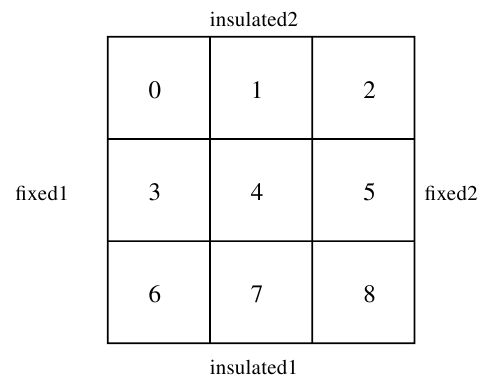
\includegraphics[width=491,height=387]{Figure4-1.png}
 % Figure4-1.png: 491x387 pixel, 96dpi, 12.99x10.24 cm, bb=0 0 368 290
 \caption{Рисунок 4.1: Геометрия и патчи в тесте транспорта скаляров (ячейки определяются числами)}
 \label{fig:4.1}
\end{figure}


\section{Приложение А}
\label{sec:PrilA}

\section{Приложение B}
\label{sec:PrilB}

\section{Приложение C}
\label{sec:PrilC}

\end{document}
